\documentclass[
,hyperref={pdfpagelabels=false}
]{beamer}
% Die Hyperref Option hyperref={pdfpagelabels=false} verhindert die Warnung:
% Package hyperref Warning: Option `pdfpagelabels' is turned off
% (hyperref)                because \thepage is undefined.
% Hyperref stopped early

\usepackage{agstyle}
\usepackage{currycode}
\usepackage{tikz}

\newcommand{\ergo}{$\Rightarrow$}
\newcommand{\todo}[1]{\fbox{\sc To do: #1}}

%%%%%%%%%%%%%%%%%%%%%%%%%%%%%%%%%%%%%%%%%%%%%%%%%%%%%%%%%%%%%%%%%%%%%%%%%%%%%%%%

\title[Search Strategies for FLP]
{Search Strategies for Functional Logic Programming}

\date[ATPS 2012]{ATPS 2012, February 27}

\author[Hanus, Peemöller, \underline{Reck}]{%
\texorpdfstring
  {Michael Hanus \and Björn Peemöller \and \underline{Fabian Reck}}
  {Michael Hanus \and Björn Peemöller \and Fabian Reck}
}

\institute{Kiel University}

\begin{document}

\begin{frame}%---------------
\titlepage
\end{frame}

%%%%%%%%%%%%%%%%%%%%%%%%%%%%%%%%%%%%%%%%%%%%%%%%%%%%%%%%%%%%%%%%%%%%%%%%%%%%%%$$

\section{Introduction}

\begin{frame}[fragile]%-------------------------------------------------------
\frametitle{Functional Logic Programming}
\begin{itemize}
\item Combines features from functional and logic Programming
  \begin{itemize}
   \item Higher-order functions
   \item Demand-driven evaluation
   \item non-determinism
   \item logic variables
  \end{itemize}
\item Search for results
\item Different strategies
\end{itemize}
\end{frame}

\begin{frame}[fragile]%------------------------------------------------------
\frametitle{Curry}
\begin{itemize}
\item Haskell like Syntax
\item Lazy evaluation
\end{itemize}
\begin{block}{KiCS2}
\begin{itemize}
\item KiCS2 is a compiler from Curry to Haskell
\item Non-determinism is explicitly represented in
      the data structures
\end{itemize}
\end{block}
\end{frame}

\begin{frame}[fragile]%-------------------------------------------------------
\frametitle{Curry}
\begin{curry}%{Example}
(?) :: a -> a -> a
x ? _ = x
_ ? y = y

coin :: Int
coin = 1 ? 2

(++) :: [a] -> [a] -> [a]
[] ++ ys = ys
(x:xs) ++ ys = x : (xs ++ ys)

last :: [a] -> a
last xs | (ys ++ [z]) =:= xs = z
  where ys, z free
\end{curry}
\begin{itemize}
\item Overlapping rules
\item Free variables
\item Constraints
\end{itemize}
\end{frame}

\begin{frame}[fragile]%-------------------------------------------------------
\frametitle{Curry implementation and their strategies}
\begin{description}
\item[PAKCS] Curry to Prolog, uses backtracking (DFS)
\item[MCC] translates to C, DFS
\item[KiCS] translates to unsafe Haskell, DFS and BFS
\item[KiCS2]translates to Haskell, DFS, BFS, IDS, PAR, easily extensible
\end{description}
\end{frame}

\section{Search Strategies}

\begin{frame}[fragile]%-------------------------------------------------------
\frametitle{Search space representation in KiCS2}
\begin{columns}[t]
\begin{column}{0.45\textwidth}
\begin{curry}
last [T,F] 
=> ys ++ [z] =:= [T,F] &> z
\end{curry}
\begin{tikzpicture}
\node (qys)   at (2,5) {$\code{?}^{\code{ys}}$};
\node (f1)    at (1,4) {$\code{!}$}           ;
\node (qx)    at (3,4) {$\code{?}^{\code{x}}$} ;
\node (qxs)   at (2,3) {$\code{?}^{\code{xs}}$};
\node (f2)    at (4,3) {$\code{!}$}           ;
\node (qz1)   at (1,2) {$\code{?}^{\code{z}}$} ;
\node (f3)    at (3,2) {$\code{!}$}           ;
\node (f4)    at (0,1) {$\code{!}$}           ;
\node (qz2)   at (2,1) {$\code{?}^{\code{z}}$} ;
\node (true)  at (1,0) {$\code{T}$}           ;
\node (false) at (3,0) {$\code{F}$}           ;
\draw (qys) -- node[sloped,above]{\tiny{$\code{[]}$}}   (f1)   ;
\draw (qys) -- node[sloped,above]{\tiny{$\code{x:xs}$}} (qx)   ;
\draw (qx)  -- node[sloped,above]{\tiny{$\code{T}$}}    (qxs)  ;
\draw (qx)  -- node[sloped,above]{\tiny{$\code{F}$}}    (f2)   ;
\draw (qxs) -- node[sloped,above]{\tiny{$\code{[]}$}}   (qz1)  ;
\draw (qxs) -- node[sloped,above]{\tiny{$\code{\_:\_}$}}(f3)   ;
\draw (qz1) -- node[sloped,above]{\tiny{$\code{T}$}}    (f4)   ;
\draw (qz1) -- node[sloped,above]{\tiny{$\code{F}$}}    (qz2)  ;
\draw (qz2) -- node[sloped,above]{\tiny{$\code{T}$}}    (true) ;
\draw (qz2) -- node[sloped,above]{\tiny{$\code{F}$}}    (false);
\end{tikzpicture}
\end{column}
\begin{column}{0.45\textwidth}
\begin{haskell}[SearchTree]
data SearchTree a 
  = None
  | One a
  | Choice (SearchTree a)
           (SearchTree a)
\end{haskell}
\begin{itemize}
\item Normal form computation to evaluate the search tree
\item Evaluation is lazy
\end{itemize}
\end{column}
\end{columns}
\end{frame}

\begin{frame}[fragile]%-------------------------------------------------------
\frametitle{Search strategies}

\begin{itemize}
  \item Based on tree representation of search space
  \item Strategies only extract values
  \item Available: depth-first, breadth-first, iterative deepening
\end{itemize}


\begin{haskell}[Depth-first-search using SearchTree]
allValuesDFS :: SearchTree a -> [a]
allValuesDFS None         = []
allValuesDFS (One      x) = [x]
allValuesDFS (Choice x y) = allValuesDFS x ++ allValuesDFS y
\end{haskell}

\end{frame}

\begin{frame}[fragile]%-------------------------------------------------------
\frametitle{Interactive exploration of the results}
\begin{haskell}
printResults :: [a] -> IO ()
printResults []     = putStrLn "No more values"
printResults (x:xs) = do print x
                         putStr "More values? "
                         inp <- getLine
                         if inp == "yes" then printResults xs
                                         else done
\end{haskell}
\begin{itemize}
\item SearchTree available in Curry
\item User defined Strategies
\item Encapsulated search
\end{itemize}
\end{frame}

\section{Benchmarks}

\begin{frame}%----------------------------------------------------------------
\frametitle{Benchmark: Non-Deterministic Permutation Sort}
Program: permutation sort of a list with 15 values
\begin{center}
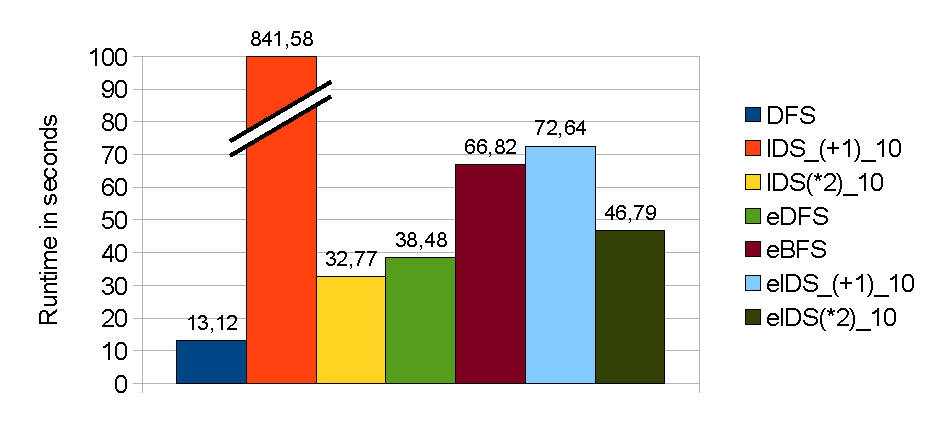
\includegraphics[width=11cm]{gfx/permsort}
\end{center}
%\begin{itemize}
%\item DFS/eDFS: Overhead durch Suchbaum, Faktor 3
%\item $\text{IDS}_{10}^{+1}$ is very slow due to the linear search space
%\item $\text{eIDS}_{10}^{+1}$ profits from sharing the search tree
%\item IDS(+1)/IDS(*2): Overhead durch Gewährleistung von CTC
%\item IDS(*2)/eIDS(*2): Overhead durch Suchbaum, Faktor 1,5
%\item IDS(+1)/eIDS(+1). \todo{Aussage}
%\end{itemize}
\end{frame}

\begin{frame}[fragile]%-------------------------------------------------------
\frametitle{Benchmark: Last}
Program: find the last element of a 10,000 element list
\begin{center}
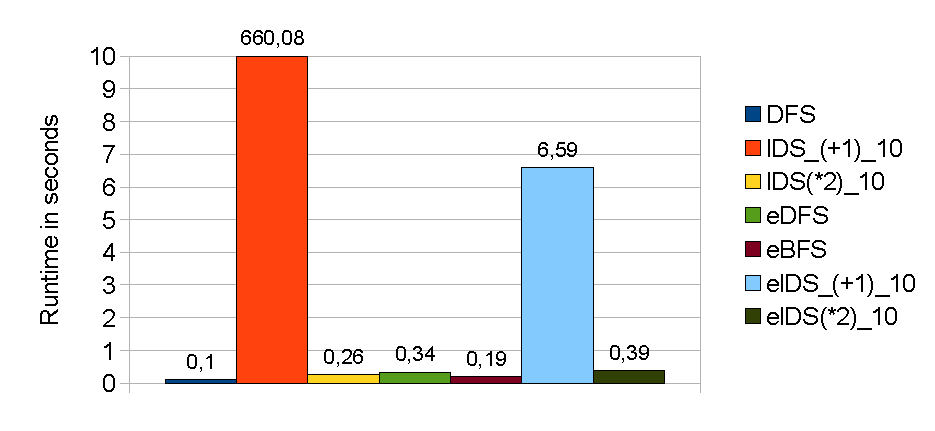
\includegraphics[width=11cm]{gfx/last}
\end{center}
% \todo{Laufzeit von BFS erklären}
\end{frame}

\begin{frame}[fragile]%-------------------------------------------------------
\frametitle{Benchmark: NDNums}

%\todo{IDS ist voll gut!}
\end{frame}

\section{Conclusion}

\begin{frame}[fragile]%-------------------------------------------------------
\frametitle{Conclusion}

\begin{itemize}
\item Presentation of our approach to search
\item First practical results
\item Avoid problems arising from the use of a fixed strategie
\item Complete strategies are realistic alternatives to DFS
\end{itemize}

\end{frame}

\begin{frame}[fragile]%-------------------------------------------------------
\frametitle{Future Work}

\begin{itemize}
\item Analysis of more complex programs
\item Analysis of memory behaviour
\item Analysis of additional (parallel) strategies
\end{itemize}

\end{frame}

\end{document}
